\documentclass{beamer}
\usepackage[utf8]{inputenc}
 \usetheme{Boadilla}
\title{Exploring the impact of language differences on GANs for password cracking}
\subtitle{Thesis Exam}
\author{Eugenio Maria Capuani}
\date{June 20th, 2019}
\usepackage{pgfplots} 
\begin{document}
\begin{frame}
\titlepage
\end{frame}

\begin{frame}
\frametitle{Contents}
\begin{itemize}
\item Overview of the thesis
\item New data addressing the problem brought up in the discussion
\item Criticisms    
\end{itemize}
\end{frame}

\begin{frame}
\frametitle{Overview of the thesis}
    \section{Introduction}
    The goal of the thesis was to explore the impact of language on GANs for password cracking: to that end, we tested PassGAN with a set of Italian Passwords (the Libero dataset).
    We also compared PassGAN with rule-based password crackers (HashCat):

Concerning the impact of language, our goal was three-fold:
    \begin{itemize}
        \item To see whether GANs are capable of learning and using language-specific features in passwords, and compare them with rule-based tools (which have no such capability).
        \item To explore the impact of training with Natural Language data.
        \item To establish whether PassGAN or similar tools offer something new and unique, if they offer us things that could not be achieved with rule-based tools.    
    \end{itemize}
\end{frame}

\begin{frame}
\frametitle{Overview of the thesis}
\section{Findings}
\begin{itemize}
    \item We found that rule-based tools are more effective than PassGAN when using the same number of password candidates, but also that PassGAN can match HashCat's performance if more password candidates can be used.
    \item We found that even when constrained to a low amount of password candidates, used in conjunction with rule-based tools PassGAN can be an effective way to tackle longer passwords with language-specific characteristics.
    \item We found that natural language does not seem to have an impact of PassGAN's performance, suggesting that training should be limited to password data only. 
    \item We found that mangling rules can be effective when used with PassGAN (in contrast to the original paper) as they improve performance with low numbers of Password candidates.
They might provide a compromise between the language optimizations provided by PassGAN.
\end{itemize}

% Ultimately we concluded that PassGAN can be an effective password-cracking tool, as it is more flexible than rule-based tools.   
\end{frame}

\begin{frame}
\frametitle{New data}

One of the topics we discussed in the Discussion was that we did not compare the cracking performance of the pre-trained PassGAN model (trained by Hitaj. et al. on English passwords) to our own model trained on Italian passwords.
\end{frame}

\begin{frame}
\frametitle{New data}
\begin{figure}[H]
\centering
    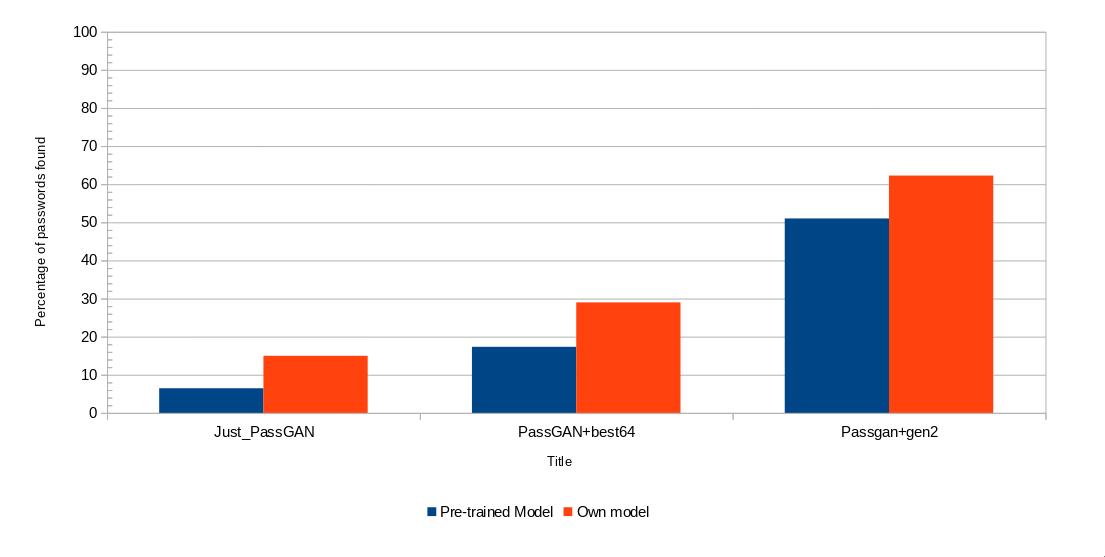
\includegraphics[scale=0.30]{chart.png}
    %\caption{A diagram illustrating our general workflow for evaluating PassGAN, including Training and Testing.}
    %\label{fig:testing_flowchart}
\end{figure}
\end{frame}    

\begin{frame}
\frametitle{Criticisms}
Most of the criticisms we have about the thesis are detailed in the discussion, however there is one point we'd like to re-iterate:

In retrospect we should have started the testing chapter with a discussion of huge wordlists and outline the strengths and weaknesses of the two approaches (HashCat and PassGAN).

We feel that setting up the section comparing the two with a small wordlist does not fully represent the capabilities of PassGAN.
\end{frame}    
\end{document}
